


\section{Algorithms}


\cite{kahnkim1} gave the the first polynomial-time algorithm achieving the bound $\BigO{\log e(P)}$ up to a constant factor in 1995. Their algorithm uses the ellipsoid algorithm to choose a good comparison at each step which makes this algorithm only of theoretical interest. 

Finally, in 2013, \cite{cardinal2013sorting}, new methods are developed. Three new algorithms having the same canvas : a first poly-time preprocessing phase followed by a $\BigO{\log e(P)}$ query phase. Caution has to be made though : each of the three different algorithms match the ITLB for a subset of the problem instances.

\begin{table}
	\begin{center}
	\caption{We denote by $E A(n)$ the time needed for the ellipsoid algorithm to compute the entropy of a poset of order $n$. The original bound given by \cite{kahnkim1} on the number of comparisons performed by their algorithm is $54.45 \cdot \log e(P)$. The improved bound given in the table is a byproduct of the results of \cite{cardinal2013sorting}. (The notation $\BigOe{n}$ means that the hidden constant may depend on $\epsilon$.)}
	\label{tree:supi:table/jcardin}
	\begin{tabular}{|c|c|c|}

	\hline
	Algorithm & Global Complexity & Number of comparisons\\\hline\hline
	\cite{kahnkim1} & $\BigO{n \log n \cdot E A(n)}$ & $\leq 9.82 \cdot \log e(P)$\\\hline\hline
	\cite{cardinal2013sorting} \textbf{1} & $ \BigO{n^{2}} $ & $\BigO{\log n \cdot \log e(P)}$ \\\hline
	\cite{cardinal2013sorting} \textbf{2} & $ \BigO{n^{2.5}} $ & $\leq (1 + \epsilon) \log e(P) + \BigOe{n}$ \\\hline
	\cite{cardinal2013sorting} \textbf{3} & $ \BigO{n^{2.5}} $ & $\leq 15.09 \cdot \log e(P)$ \\\hline

	\end{tabular}
	\end{center}
\end{table}


\ref{tree:supi:table/jcardin} highlights the properties of the different algorithms, i.e.

\begin{itemize}

\item If $\log e(P)$ is super-linear in $n$, the number of comparisons of \cite{cardinal2013sorting} \textbf{2} is lower than that of \cite{kahnkim1}. By optimizing over $\epsilon$, it can be shown that the number of comparisons is actually $\log e(P) + \SmallO{\log e(P)} + \BigO{n}$ in this case, a number of comparisons comparable to that of Fredman’s algorithm.

\item If $\log e(P)$ is linear or sub-linear in $n$, the number of comparisons of \cite{cardinal2013sorting} \textbf{3} is comparable to that of \cite{kahnkim1}, although the constant in front of $\log e(P)$ is still far from the best constant achieved by a super-polynomial algorithm via balancing pairs \cite{brightwell1995balancing, brightwell1999balanced}.

\item Algorithms from \cite{cardinal2013sorting} have the following useful property: they compute information that guides the sorting and can then be reused to solve any given instance with the same partial information $P$, in time proportional to the number of comparisons, plus a term linear in $n$.

\end{itemize}


Looking at \ref{fig:supi/alg2}, algorithm 2 looks like to what is done in \cite{jcardin1} for the Partial Order Production problem if we swap the roles of chains and antichains. This is explained in detail in \cite{DBLP:conf/birthday/CardinalF13}.


\begin{figure}
	\centering
	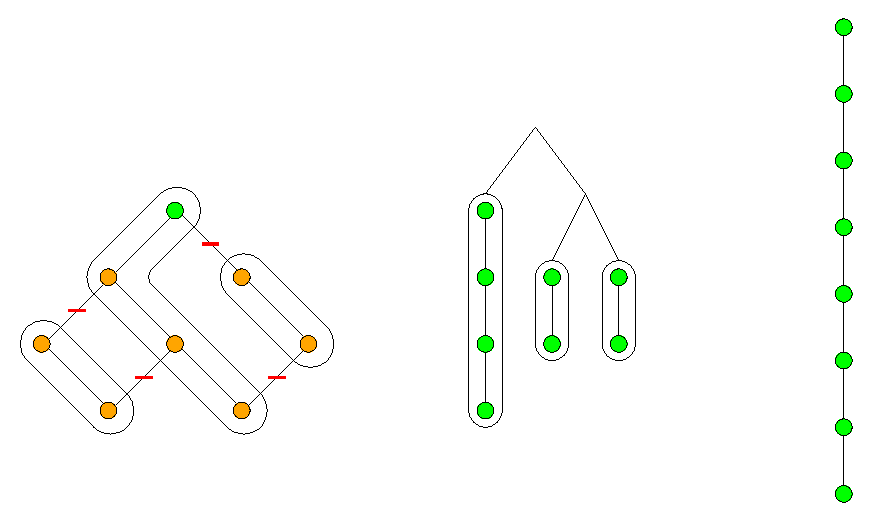
\includegraphics[height=0.2\textheight]{fig/supi/reduction:diag}
	\caption{\label{fig:supi/alg2} Illustration of the second algorithm in \cite{cardinal2013sorting}.}
\end{figure}


Note that randomized algorithms also exist for this purpose. The idea is to evaluate the quality of a comparison by generating a sample of possible linear extensions, count the number of times the answer to this question ``$x \stackrel{?}{\le} y$'' is true and then only ask the question if the ratio of this count over the total number of sampled linear extensions lies within a fixed interval $[q, 1-q], 0 < q \le \frac{1}{3}$. See \cite{huber2006fast} for more.

